%sample content to demonstrate LaTeX command.
\vspace{21.5pt}
\chapter{Demonstration Content}\label{demo:content}

This is a chapter to demonstrate some of the \gls{latex} commands that you can use to format your text. If you are new to it, \gls{latex} follows the \gls{wysiwym} idea similar to \gls{html} where you concentrate on the content and structure and leave the formatting and styling to the computer. You will write your content in a plain text file\footnote{which can not get corrupted and can be put under version control} and indicate the structure with commands (similar to \gls{html} tags) then compile it to generate the pdf. Check some books or tutorials such as \LaTeX{} Wikibooks\footnote{\url{https://en.wikibooks.org/wiki/LaTeX}} and try with an online editor such as Overleaf\footnote{\url{https://www.overleaf.com/}} so you do not need to install the compiler on your computer first.

\section{Text, terms and abbreviations, figures, lists, etc.}

In \gls{latex}, the \mintinline{tex}{\textbf{bold}} command produces \textbf{bold}, \mintinline{tex}{\textit{italic}}  \textit{italic} and nesting \mintinline{tex}{\textbf{\textit{bolditalic}}} generates \textbf{\textit{bolditalic}}. If the goal is to semantically mark importance, then use \emph{emphasize} with \mintinline{tex}{\emph{emphasize}} command. That would take care of cases such as \mintinline{tex}{\textit{text in italic with \emph{important stuff} inside}} which will compile to \textit{text in italic with \emph{important stuff} inside}. Note that a paragraph is added by forcing a new line.

When one want to use an abbreviation or acronym like \gls{html} using the \mintinline{tex}{\gls{html}} command in \gls{latex}, the first time, it comes with it full version as can be seen in first paragraph of chapter \ref{demo:content} and for all next usages in its short form. Of course, when needed, the full version is available using e.g. the \mintinline{tex}{\acrlong{someID}} command. The defined terms like \gls{maths} use the same \mintinline{tex}{\gls{math}} \gls{latex} command. The Capitalized can be obtained with \mintinline{tex}{\Gls{id}}.

In this template, the abbreviations are defined in the \texttt{chapters/0abbr.tex} file with the \mintinline{tex}{\newacronym{id}{SHORT}{Long Form}} command. There can be many abbreviations and terms defined there, only the ones that are used in the text will be printed in the list of abbreviations (after table of content). And of course, it is the job of the compiler to sort them alphabetically. Should be avoided; but to have all the abbreviations and terms, even the non-used ones, use the \mintinline{tex}{\glsaddall} command before printing the list of abbreviations.

\begin{itemize}
  \item Check the thesis guide about the orphan list item (\mintinline{tex}{\item}): if only first item in the page, force a new page \mintinline{tex}{\clearpage} before \mintinline{tex}{\begin{itemize}}.
  \item When the list items are not sentences, they begin with a lowercase letter, and the last list item ends in a period.
  \item When the list items are sentences, they begin with a capitalized letter, and the list items end in a period. If item of the list contains a long text that spans multiple lines, the left edge aligns automatically.
\end{itemize}

And let also try the figure (see figure \ref{fig:latex-cover}) and internal reference (with \mintinline{tex}{\label{lbl:id}} and \mintinline{tex}{\ref{lbl:id}}). Alternative text is obtained with custom made \mintinline{tex}{\AltText{text}} command (using pdfcomment and accsupp packages). The reference can be done to any label, for example why not to appendix \ref{appx:first} or to appendix \ref{appx:second}? To note, \gls{latex} will place the figure to the best place (except with forcing). Let them float till the final of final edit\ldots ~then force them to not break a paragraph.%hugly hack... I'm sorry

\begin{figure}[ht]
  \centering
  \AltText{meaningful alternative description (e.g. LaTeX, from typeseting to genrated pdf)}{
\includegraphics[width=7.1cm]{LaTeX_cover}}
  \caption{\gls{latex} cover image (Copied from \citeauthor{wikibooks:latex} (\citedate{wikibooks:latex}) \cite{wikibooks:latex}).}
  \label{fig:latex-cover}
\end{figure}

According to the thesis guide, there must be a paragraph of text between figures/tables/listings and a chapter/(sub)section. And a paragraph is many sentences long like at least two.

\section{Bibliography references and citations}

Here is an example how to cite a bibliography entry \cite{kopka:guide} using the \\\mintinline{tex}{\cite{kopka:guide}} \gls{latex} command \cite[section 4.1]{tobias:book}. You might also like \mintinline{tex}{\citeauthor{some:id}} and \mintinline{tex}{\citedate{some:id}} ~as demonstrated in figure \ref{fig:latex-cover} caption and others like \mintinline{tex}{\citetitle{some:id}}, \mintinline{tex}{\citeurl{some:id}}, etc. To get very precise references, like chapter, section, pages number or range of a book, timing in video,\ldots that get indicated in square brackets in the command like \mintinline{tex}{\cite[04:01]{youtube:biblatex}} \cite[04:01]{youtube:biblatex}. Check the thesis guide, if the reference is only for the current sentence, the \mintinline{tex}{\cite{}} is placed before the dot, if the reference is for entire paragraph or group of sentences, then after the dot. If there is multiple sources for one sentence or paragraph, they have to be grouped together using the \mintinline{tex}{\cites[pp. 3, 5, 9--13]{some:id}[chap 4]{other:id}{more:id}{etc:id}} command. \cites[pp. 216--220]{kopka:guide}[chapter Special Pages, sections 3--4]{wikibooks:latex}[section 4.1]{tobias:book}[04:01--04:19]{youtube:biblatex}

Like for abbreviations, the bibliography entries are stored in a separated \texttt{biblio.bib} file and only the \mintinline{tex}{\cite}d ones will be printed in the bibliography references. There are many entry types such as \mintinline{tex}{@book}, \mintinline{tex}{@article}, \mintinline{tex}{@online}, \mintinline{tex}{@video}, \mintinline{tex}{@thesis} and many more, e.g. see \cite[section 2.1]{ctan:biblatex}. In the worst case, there is the \mintinline{tex}{@misc} fallback entry type. \gls{latex} and biber compilers will take care of the numbering and sorting of the cited entries. Some tools help in managing the entries such as OttoBib\footnote{\url{http://www.ottobib.com/}} that will generate book entry from \gls{isbn} or ZoteroBib\footnote{\url{https://zbib.org/}} that can also take \gls{url}, \gls{doi}, etc. It is also possible to get the entry form the IEEE Xplore\footnote{\url{https://ieeexplore.ieee.org/}} or Google Scholar\footnote{\url{https://scholar.google.com/}} as shown in figure \ref{fig:bibtex}. Of course, even if using such tools can greatly help, manual check/edit might be required (e.g. missing author,\ldots).

\begin{figure}[ht]
  \centering
  \AltText{getting BibTeX entries from Google Scholar and IEEE Xplore}{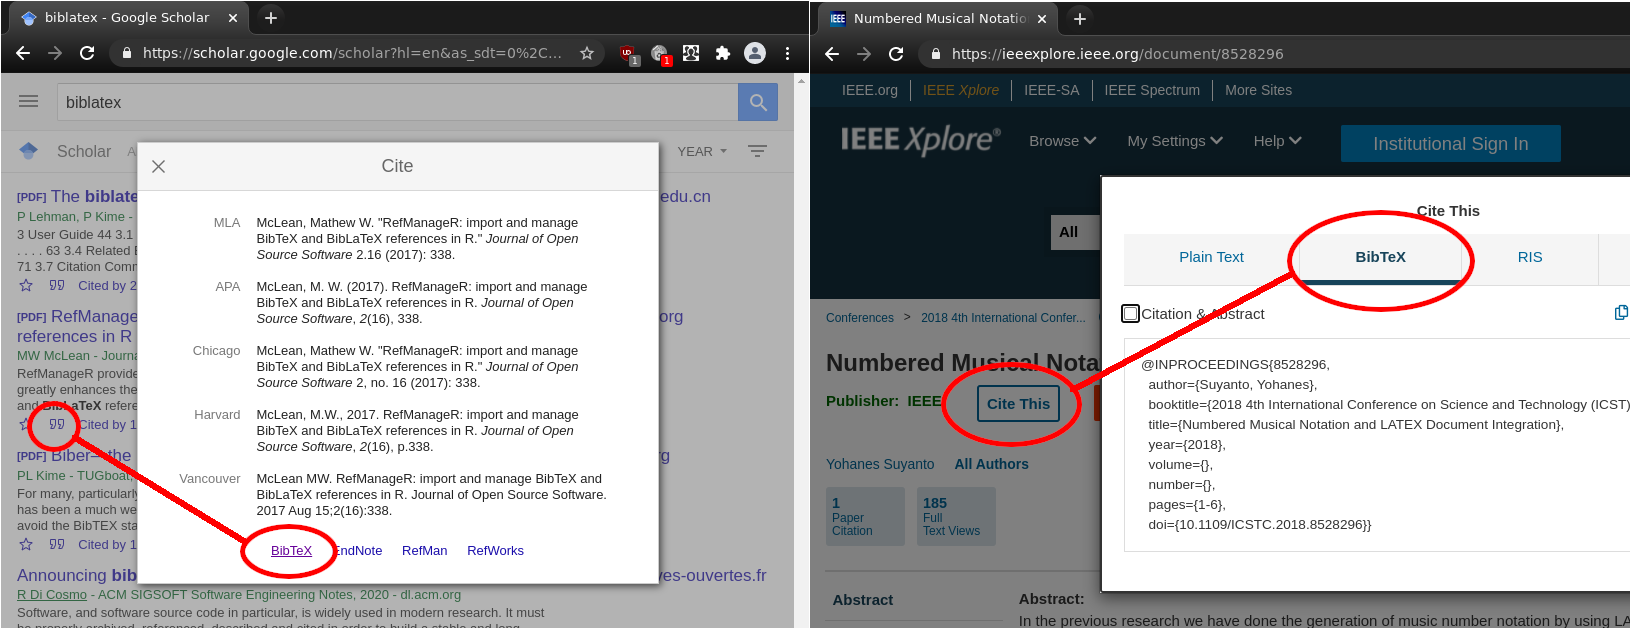
\includegraphics[width=\textwidth]{bibtex_gscholar_ieeexplore}}
  \caption{BibTeX entries from Google Scholar (left) or IEEE Xplore (right)}
  \label{fig:bibtex}
\end{figure}

Let's also try a long quote from the \citetitle{un:udhr}
\begin{quote}
(1) Everyone has the right to education. Education shall be free, at least in the elementary and fundamental stages. Elementary education shall be compulsory. Technical and professional education shall be made generally available and higher education shall be equally accessible to all on the basis of merit.

(2) Education shall be directed to the full development of the human personality and to the strengthening of respect for human rights and fundamental freedoms. It shall promote understanding, tolerance and friendship among all nations, racial or religious groups, and shall further the activities of the United Nations for the maintenance of peace.

(3) Parents have a prior right to choose the kind of education that shall be given to their children. \cite[article 26]{un:udhr}
\end{quote}

%TODO example with cite interview/conversation (unpublished or misc)
%https://tex.stackexchange.com/questions/111363/exclude-fullcite-citation-from-bibliography
\textit{Quisque augue} est, \textbf{elementum ac porttitor} non, porttitor ac orci. Donec hendrerit, ligula ac luctus egestas, sem dolor pretium nunc, sed vehicula magna diam a massa. Donec mattis, arcu et tempor mattis, risus tortor ultrices metus, nec sodales sem dolor eu elit.

Nullam egestas enim at odio pellentesque bibendum.

\subsection{Subsection}
Donec et sapien ac leo condimentum vulputate id et tellus. Maecenas hendrerit malesuada interdum. Aenean dignissim sem faucibus elit congue faucibus id non risus. Morbi at dui non tortor pellentesque consequat non eget urna. Cras in sapien dui, a tincidunt velit.
\reaction{\label{eq:reaktio}$\underset{\text{+II}}{\ce{2Fe^2+}}$ + $\underset{\text{+I\;-I}}{\ce{H2O2}}$ + $\underset{\text{+I\;-II}}{\ce{2H3O^+}}$ <=> $\underset{\text{+III}}{\ce{2Fe^3+}}$ + $\underset{\text{+I\;-II}}{\ce{4H2O}}$}
Työn aluksi rauta(II)ionit hapetetaan rauta(III)ioneiksi väkevällä vetyperoksidilla, kuten reaktion~\ref{eq:reaktio} hapetusluvuista nähdään (rauta hapettuu, happi pelkistyy).
\reaction{Fe^3+( \emph{aq} ) + 3OH^-( \emph{aq} ) + $(x-1)$H2O( \emph{l} ) -> FeOOH $\cdot$ $x$(H2O)( \emph{s} )}
Rauta(III)ionit saostetaan emäksen (\ce{NH3}) avulla ja saadaan tuotteeksi kidevedellinen rauta(III)hydroksidi. Saatu saostuma pestään \ce{NH4NO3}:lla.
\reaction{FeOOH $\cdot$ $x$(H2O)( \emph{s} ) ->T[$\Delta$900-1000\celsius] Fe2O3( \emph{s} )}

\subsection{Subsection with \texorpdfstring{\Gls{maths}}{Mathematics}}%gls inside chapter/section/... will generate hyperref warning (link inside link in table of content), to avoid that, use the \texorpdfstring
Donec et sapien ac leo condimentum vulputate id et tellus. Maecenas hendrerit malesuada interdum. Aenean dignissim sem faucibus elit congue faucibus id non risus. Morbi at dui non tortor pellentesque consequat non eget urna. Cras in sapien dui, a tincidunt velit. Tertiäärinen butyylikloridi reagoi veden kanssa oheisen reaktion mukaisesti:
\reaction{(CH3)3CCl + 2H2O -> (CH3)3COH+H3O+ +Cl-}
Kyseessä on ensimmäisen kertaluvun reaktio, joten reaktion nopeus on
\begin{align}
v=-\frac{\mathrm{d}[\tn{t-ButCl}]}{\mathrm{d}t}=\frac{\mathrm{d}[\tn{HCl}]}{\mathrm{d}t}=k[\tn{t-ButCl}]
\end{align}
Jos tarkastellaan lähtöaineen t-butyylikloridin häviämistä saadaan
\begin{align}
\frac{\mathrm{d}[\tn{t-ButCl}]}{[\tn{t-ButCl}]}&=-k\mathrm{d}t \\
\int \frac{\mathrm{d}[\tn{t-ButCl}]}{[\tn{t-ButCl}]}&=-k \int \mathrm{d}t \\
\ln \int_{[\tn{t-ButCl}]_0}^{[\tn{t-ButCl}]} [\tn{t-ButCl}]&=-k\int_0^t t \\
\ln \left( \frac{[\tn{t-ButCl}]}{[\tn{t-ButCl}]_0} \right)&=-kt
\end{align}
Ionivahvuus lasketaan kaavalla.
\begin{align}
I&=\frac{1}{2}\cdot\sum z_i^2c_i \\
z_i&= \tn{ionin varausluku} \nonumber \\
c_i&= \tn{ionin konsentraatio} \nonumber
\end{align}
Aktiivisuuskerroin $\gamma_\pm$ lasketaan kaavalla.
\begin{align}
\log \gamma_\pm &= -\left|z_+\cdot z_-\right|A\cdot I^{\frac{1}{2}} \\
A &= \tn{0,509 (lämpötilassa 25\celsius}) \nonumber \\
I &= \tn{ionivahvuus} \nonumber \\
z &= \tn{ionien varaus} \nonumber
\end{align}

\section{Section with Source Code}
Donec et sapien ac leo condimentum vulputate id et tellus. Maecenas hendrerit malesuada interdum. Aenean dignissim sem faucibus elit congue faucibus id non risus. Morbi at dui non tortor pellentesque consequat non eget urna. Cras in sapien dui, a tincidunt velit.

%For sharelatex users, use space instead of tab to avoid ^^I
\begin{code}
  \begin{minted}{php}
<?php
$username = $_POST["username"];
//maybe not?
if ($userName){
  ?>
  <h2>Hello <?= $username ?>!</h2>
  <p>your message got received.</p>
  <?php
}
?>
\end{minted}
\captionof{listing}{Descriptive Caption Text (e.g. this \gls{php} code do blah)}
  \label{code:testphp}
\end{code}


As see in listing \ref{code:testphp}, blah. It is also possible to have code inline, for example \mintinline{sql}{SELECT * FROM user WHERE age >= 18} that was \gls{sql}.
The lisings \ref{code:htmlfull} and \ref{code:htmlpart} show how to load code from an external source file. In the case of listing \ref{code:htmlpart} it only take few line out of the source code file.

\begin{code}
  \inputminted{html}{code/html5_sample.html}
  \captionof{listing}{Some \gls{html} code}
  \label{code:htmlfull}
\end{code}
 Donec et sapien ac leo condimentum vulputate id et tellus. Maecenas hendrerit malesuada interdum. Aenean dignissim sem faucibus elit congue faucibus id non risus.

 \begin{code}
   \inputminted[firstline=3,lastline=6]{html}{code/html5_sample.html}
   \captionof{listing}{The \mintinline{html}{<head>} section of an \gls{html} page}
  \label{code:htmlpart}
\end{code}


 Morbi at dui non tortor pellentesque consequat non eget urna. Cras in sapien dui, a tincidunt velit.


\section{Section with Table}
Donec et sapien ac leo condimentum vulputate id et tellus. Maecenas hendrerit malesuada interdum. Aenean dignissim sem faucibus elit congue faucibus id non risus. Morbi at dui non tortor pellentesque consequat non eget urna. Cras in sapien dui, a tincidunt velit.

\begin{table}[h]
  \centering
  \caption{Some data}%IMPORTANT the caption must be before the tabular, so it will be on top of the table (there are other tricks to force it on top; but this one is straightforward).
  \vspace{-16.5pt}%time to time, spacing between caption and table can go too big...
  \begin{tabular}{| l | >{\centering\arraybackslash}p{.5\textwidth} |}
    \hline
    Test 1 & test 1234 test \\
    \hline
    Some more data comes here & with more values and if the text is very long it will disappear out of the box unless you force the column size :( You can use e.g. \textbackslash raggedright or \textbackslash centering (as in this example) to avoid hyphenization of long words\ldots \\
    \hline
  \end{tabular}
  \label{table:some_data}
\end{table}

As presented in table \ref{table:some_data}: Donec et sapien ac leo condimentum vulputate id et tellus. Maecenas hendrerit malesuada interdum. Aenean dignissim sem faucibus elit congue faucibus id non risus. Morbi at dui non tortor pellentesque consequat non eget urna. Cras in sapien dui, a tincidunt velit.

\begin{table}[h]
  \centering
  \caption{Another table with tabularx}
  \begin{tabularx}{.95\textwidth}{| l | >{\centering\arraybackslash} X |}
    \hline
    Test 1 & test 1234 test \\
    \hline
    Some more data comes here & with more values and if the text is very long it will disappear out of the box unless you force the table size :( \\
    \hline
  \end{tabularx}
  \label{table:some_data2}
\end{table}

As presented in table \ref{table:some_data2}: Donec et sapien ac leo condimentum vulputate id et tellus. Maecenas hendrerit malesuada interdum. Aenean dignissim sem faucibus elit congue faucibus id non risus. Morbi at dui non tortor pellentesque consequat non eget urna. Cras in sapien dui, a tincidunt velit.

Donec et sapien ac leo condimentum vulputate id et tellus. Maecenas hendrerit malesuada interdum. Aenean dignissim sem faucibus elit congue faucibus id non risus. Morbi at dui non tortor pellentesque consequat non eget urna. Cras in sapien dui, a tincidunt velit.

\begin{table}[htbp]
  \centering
  \caption{Booktabs example}
  \vspace{-16.5pt}
    \begin{tabular}{rrrr}
    \toprule
    t (s) & [HCl] & [t-ButCl] & $\ln\frac{[t-ButCl]}{[t-ButCl]_0}$ \\
    \midrule
    0     & 4,02  & 160,88 & 0,00 \\
    10    & 63    & 101,9 & -0,46 \\
    20    & 115,2 & 49,7  & -1,17 \\
    30    & 141,3 & 23,6  & -1,92 \\
    40    & 157,9 & 7     & -3,13 \\
    50    & 161   & 3,9   & -3,72 \\
    60    & 164,3 & 0,6   & -5,59 \\
    70    & 163,5 & 1,4   & -4,74 \\
    80    & 163,8 & 1,1   & -4,99 \\
    90    & 164,1 & 0,8   & -5,30 \\
    100   & 164,3 & 0,6   & -5,59 \\
    \bottomrule
    \end{tabular}
  \label{tab:thisislabel}
\end{table}

As presented in table \ref{tab:thisislabel}: Donec et sapien ac leo condimentum vulputate id et tellus. Maecenas hendrerit malesuada interdum. Aenean dignissim sem faucibus elit congue faucibus id non risus. Morbi at dui non tortor pellentesque consequat non eget urna. Cras in sapien dui, a tincidunt velit.
